% This is samplepaper.tex, a sample chapter demonstrating the
% LLNCS macro package for Springer Computer Science proceedings;
% Version 2.20 of 2017/10/04
%
\documentclass[runningheads]{llncs}
%
\usepackage{graphicx}
\usepackage{authblk}
\usepackage{subfigure}
\usepackage[section]{placeins}
\usepackage[portuguese]{babel}
\usepackage{longtable}

% Used for displaying a sample figure. If possible, figure files should
% be included in EPS format.
%
% If you use the hyperref package, please uncomment the following line
% to display URLs in blue roman font according to Springer's eBook style:
% \renewcommand\UrlFont{\color{blue}\rmfamily}

\begin{document}
%
\title{Resolução de um problema de decisão usando Programação em Lógica com Restrições: Gold Star}
%
\titlerunning{Resolução de problema Gold Star}
% If the paper title is too long for the running head, you can set
% an abbreviated paper title here
%
\author{Filipe Recharte\orcidID{up201806743}}
\author{Rita Peixoto\orcidID{up201806257}}
\authorrunning{Filipe Recharte e Rita Peixoto}
\affil{FEUP-PLOG, Turma 3MIEIC05, Grupo Gold Star\_2}

\date{4 de janeiro de 2021} 

\institute{Faculdade de Engenharia da Universidade do Porto}

%
\maketitle              % typeset the header of the contribution
%
\begin{abstract}
Descrição da resolução de um problema de decisão que consiste num puzzle, Gold Star, usando programação em lógica com restrições, com o desenvolvimento da solução em SICStus Prolog. Exploram-se as variáveis de decisão e as restrições aplicadas, com descrição da solução desenvolvida e análise das conclusões dos diversos testes. Foram testadas diferentes dimensões e estratégias de pesquisa.

\keywords{Prolog \and Restrições \and SICStus  \and Problemas de Decisão \and  clpfd \and  Gold Star}
\end{abstract}

% possível usar \input ou \include em baixo
\section{Introdução}

No âmbito da unidade curricular de Programação em Lógica, foi proposta a construção de um programa na linguagem Prolog para a resolução de um problema de decisão, com recurso à programação em lógica com restrições, utilizando a biblioteca clpfd. 

O grupo escolheu o puzzle Gold Star, que consiste num conjunto de equações válidas exibidas em forma de estrela. 
Este trabalho divide-se em duas grandes partes que são a pesquisa da solução para problema e a geração aleatória de problemas.

O presente artigo começa por descrever o problema, passando para a abordagem na resolução do mesmo, onde é possível encontrar as variáveis de decisão, as restrições e a geração de problemas. Após isto aborda-se a visualização das soluções, é feita a análise dimensional do problema e são analisadas diferentes estratégias de pesquisa. Terminando com as conclusões a partir dos dados obtidos.

\section{Descrição do Problema}

\paragraph O problema da Gold Star consiste num puzzle que exibe um conjunto de equações em forma de estrela cujo objetivo é preencher os círculos vazios das equações de modo a que estas se tornam verdadeiras quando lidas da esquerda para a direita. A resolução do problema é preencher com operadores aritméticos (+, - , *, /) e dígitos de 0 a 9 os círculos vazios da estrela, sendo que cada dígito é utilizado uma única vez. Sendo o caso base uma estrela de 5 pontos, existem 5 equações que partilham as 10 varáveis numéricas e os 10 operadores aritméticos, obtendo uma estrela como a que se apresenta na Figura \ref{fig:configuracao_estrela_5_pontas} .

\begin{figure}[!htb]
\hfill
\subfigure[não resolvida]{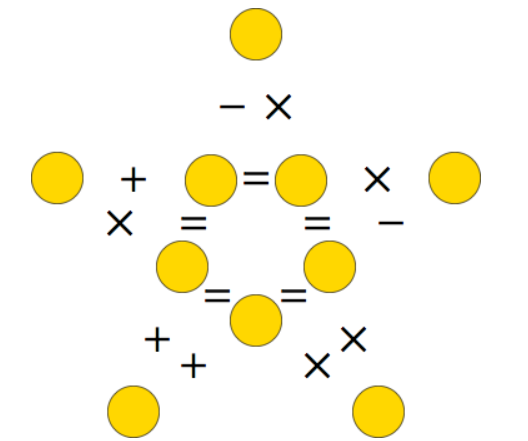
\includegraphics[width=6.4cm]{images/estrela_inicial.png}}\label{fig1}
\hfill
\subfigure[resolvida]{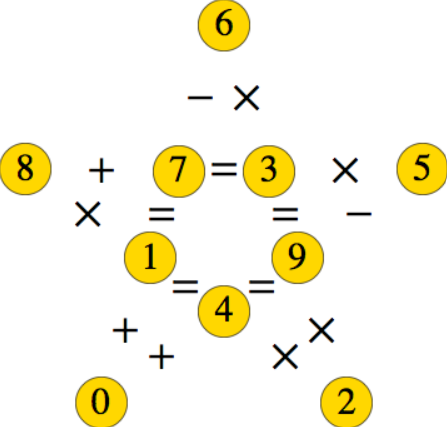
\includegraphics[width=5cm]{images/star_solved.png}}
\hfill
\caption{Exemplo da configuração da estrela de 5 pontas}\label{fig:configuracao_estrela_5_pontas}
\end{figure}




\section{Abordagem}
O puzzle Gold\_Star corresponde a um problema de satisfação de restrições (PSR). A solução de um problema de satisfação de restrições consiste na atribuição de um valor a cada variável de decisão, dentro do seu domínio, de forma a que todas as restrições sejam satisfeitas.
 
Para solucionar este problema, a estrela foi convertida num sistema de equações. Recebendo um determinado conjunto de operadores e tendo em atenção que há variáveis partilhadas entre equações, é necessário determinar valores numéricos, que substituídos nos locais vazios tornam todas as equações verdadeiras.

 
\subsection{Variáveis de decisão}
A solução do problema é constituída por duas listas, uma composta pelos operadores aritméticos, que são um de entre os seguintes: [ +, -, *, /] e outra pelos dígitos cujo domínio é [0,9].

Inicia-se a solução com a obtenção da lista de operadores do problema através do predicado getOperatorsRestricted/2 ou getOperatorsNotRestricted/2, sendo que  para tomar fazer uso da programação em lógica com restrições estes são convertidos numa representação numérica passando o seu dominío a ser [1,4], uma vez que a biblioteca clpfd apenas funciona com domínios finitos. Este predicado tem 10 variáveis de decisão, correspondendo a cada operador, no caso base do problema que são 5 pontas.

O predicado star/4 recebe a lista de operadores referida acima, traduzida para sua representação real através do predicado numberOperatorsToSignals(Ops,Operators)/2, e encontra, se possível, a solução do problema com este conjunto de operadores. Este predicado possui outras 10 variáveis de decisão, no caso base do problema, correspondendo a cada dígito.
 

\subsection{Restrições}
Todas as restrições deste problema são rígidas.
De modo a responder ao problema proposto, foi utilizado o predicado all\_distinct/1 para garantir que cada valor numérico era apenas utilizado uma única vez. Para além disso, foi implementado o predicado restrictions/6 que recebe os 2 operadores e os 4 dígitos que vão constituir uma equação e garante que esta é verdadeira com esses valores.


Sendo o problema em forma de estrela, há várias formas de gerar simetrias, desde eixos de reflexão a rotações, e portanto, tentar encontrar as soluções para este problema sem restrições iria gerar um conjunto de soluções que eram semelhantes tendo apenas uma organização diferente. Podendo estas soluções ser obtidas a partir de uma só destas soluções, por via de rotações e reflexões, é, então, escusado guardar estas soluções.

As restrições implementadas foram:
\begin{itemize}
  \item O primeiro operador da lista de operadores é o que tem o valor mais alto da lista na sua representação numérica:
  
  Com recurso ao predicado check/2, que garante que não são admitidas listas de operadores de soluções que apenas são shifts ou reflexões de outra solução, admitindo apenas a solução cujo primeiro operador é o mais elevado em termos de representação numérica. 
  
  Exemplo:
  
  1)
  
  Ops: [3,1,1,1,1,1,3,1,1,1]
  
  Vars:[4,7,2,3,8,6,0,5,9,1]
  
  
  2)
  
  Ops: [1,1,3,1,1,1,1,1,3,1]  
  
  Vars: [4,7,2,3,8,6,0,5,9,1] 
  
  
  3)
  
  Ops: [1,1,1,1,1,3,1,1,1,3] 
  
  Vars: [9,5,0,6,8,3,2,7,4,1]
  
  Neste exemplo, utilizando a restrição check, apenas a primeira opção seria aceite.
  
  \item Todas as divisões calculadas são inteiras, não sendo permitidos arredondamentos para o inteiro mais próximo. Numa fase inicial deste trabalho, foram encontradas soluções que não eram exatamente verdadeiras, uma vez que eram efetuados arredondamentos, sendo obtidas "falsas" igualdades.
\end{itemize}

Ambas estas restrições mostram reduzir bastante o espaço de solução e tempo de procura de soluções em comparação com apenas ter implementado as restrições base do problema, como é possível analisar na Tabela \ref{tab:tabela_restricoes}.

% Table generated by Excel2LaTeX from sheet 'Folha1'
\begin{table}[htbp]
  \centering
  \caption{Valores dos testes de restrições para uma estrela de 5 pontas} 
    \begin{tabular}{lrr} \hline
          & \multicolumn{1}{l}{\textbf{Tempo de execução(ms)}} & \multicolumn{1}{l}{\textbf{Número de soluções obtidas}} \\ \hline
    \textbf{sem restrições} & 234494 & 1516944 \\
    \textbf{com check} & 417620 & 784598 \\
    \textbf{com divisão} & 1118504 & 5071 \\
    \textbf{com check e divisão} & 80254 & 838 \\ \hline
    \end{tabular}%
  \label{tab:tabela_restricoes}%
\end{table}%


\subsection{Geração de problemas}
Como referido anteriormente, este trabalho integra, também,a geração de problemas a resolver. Neste caso, a implementação é em tudo semelhante diferindo apenas a forma como são geradas as listas de operadores, que passam a ter uma geração pseudo-aleatória. Tal acontece dando uso ao predicado getOperatorsRandom/2 que gera os operadores, depois é testado o solver e se tiver solução termina, senão vai gerar uma nova configuração de operadores e tenta arranjar uma solução para esta configuração, dando uso ao predicado repeat. 

  % Table generated by Excel2LaTeX from sheet 'Folha1'
\begin{table}[htbp]
  \centering
  \caption{Tempo médio de execução da procura de uma solução para uma configuração de operadores gerada de forma pseudo-aleatória}
    \begin{tabular}{lr} \hline
    \textbf{N º de pontas} & \multicolumn{1}{l}{\textbf{Tempo de execução(ms)}} \\ \hline
    \textbf{3 not restricted} & 0,666666667 \\
    \textbf{3 restricted} & 0,666666667 \\
    \textbf{4 not restricted} & 9 \\
    \textbf{4 restricted} & 34,33333333 \\
    \textbf{5 not restricted} & 24 \\
    \textbf{5 restricted} & 28,66666667 \\
    \textbf{6 not restricted} & 129 \\
    \textbf{6 restricted} & 197,3333333 \\ \hline
    \end{tabular}%
  \label{tab:tabela_random}%
\end{table}%



Na Tabela \ref{tab:tabela_random}, analisando o tempo médio das diferentes tentativas para o mesmo caso, é possível concluir que com o aumento da dimensão do problema  aumenta o tempo de execução da procura.


\section{Visualização da Solução}

O predicado print\_gold\_star/2 é utilizado para a representação de uma solução quando a estrela é constituída por 5 pontas, uma vez que é o tamanho padrão deste problema (Figura \ref{fig: print_gold_star}). Para dimensões superiores, seria necessário fazer uma função por tamanho, não sendo relevante para este trabalho.

\begin{figure}[!htb]
\hfill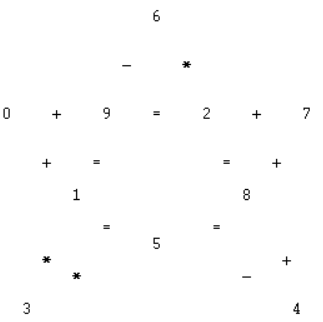
\includegraphics[width=6cm,height=6cm]{images/print_gold_star.png}\hspace*{\fill}
\caption{Exemplo do output na consola do predicado print\_gold\_star para uma solução de uma estrela de 5 pontas} \label{fig: print_gold_star}
\end{figure} 

Quando se pretende encontrar solução para uma estrela com tamanho diferente de 5, são impressas duas listas, uma com os operadores, outra com os operandos que correspondem a uma solução válida, recorrendo ao predicado print\_solution/2 (Figura \ref{fig: print_solution} ).




\begin{figure}[!htb]
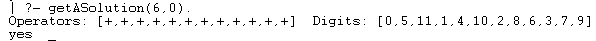
\includegraphics[width=\textwidth]{images/print_solution.png}
\caption{Exemplo do output na consola do predicado print\_solution para uma solução de uma estrela de 6 pontas} \label{fig: print_solution}
\end{figure}

A organização da lista de operadores e da lista de operandos está de acordo com a Figura \ref{fig: organizacao_estrela} .

\begin{figure}[!htb]
\hfill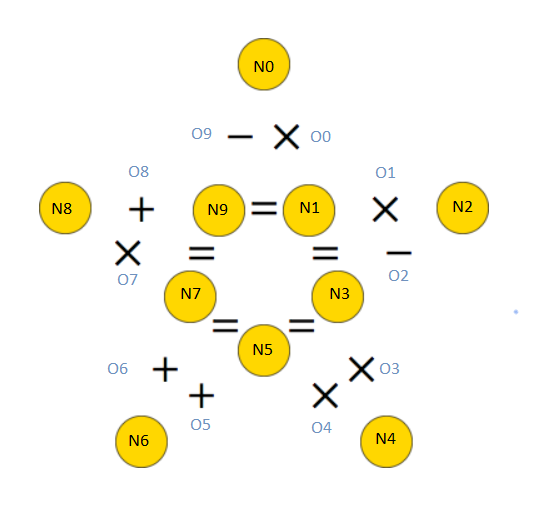
\includegraphics[width=7cm,height=7cm]{images/star_configuration.png}\hspace*{\fill}
\caption{Organização da lista de operadores e da lista de operandos para uma estrela de 5 pontas} \label{fig: organizacao_estrela}
\end{figure}

O programa contém dois predicados gerais, um para obter soluções e estas serem escritas para a consola, run/3, que recebe o predicado a ser chamado, bem como a dimensão do problema e se deve ser aplicada a restrição de check ou não, e outro para escrever para um ficheiro as soluções obtidas, save/4, que recebe o predicado a ser chamado, o nome do ficheiro em que vão ser guardadas as soluções, a dimensão do problema e se deve ou não ser aplicada a restrição check.
O predicado a ser chamado pode ser getASolution/2 que obtém uma solução para uma configuração de operaores, getConfigurationSolution/2 que obtém uma solução para cada configuração de operadores possível, getAllSolutions que obtém todas as soluções para cada configuração de operadores possível e getRandomSolution que obtém uma solução para a configuração aleatória de operadores com solução.


\section{Experiências e resultados}

\subsection{Análise Dimensional}
Após chegar à ideia base deste problema de o traduzir num sistema de equações, facilmente se pode aumentar a dimensão do problema, que, em termos visuais, é o acréscimo de uma ponta à estrela e, em termos do sistema de equações, é o acréscimo de uma equação. A adição desta nova equação exige, por sua vez, a adição de uma nova restrição.

Para responder à análise dimensional para além das restrições fixas encontradas, que são o caso do sistema de equações caso seja uma estrela de 3 pontas, que é a dimensão mais pequena possível, são também impostas restrições que variam com o tamanho da estrela, podendo desde já se concluir que o número de restrições aumenta linearmente com a dimensão.

De modo a implementar estas restrições foram criados os predicados fixed\_restrictions/3 e growing\_restrictions/3, em que o primeiro aplica as mesmas restrições em qualquer caso e o segundo lida com este aumento de uma equação por ponta adicionada.

\begin{figure}[!htb]
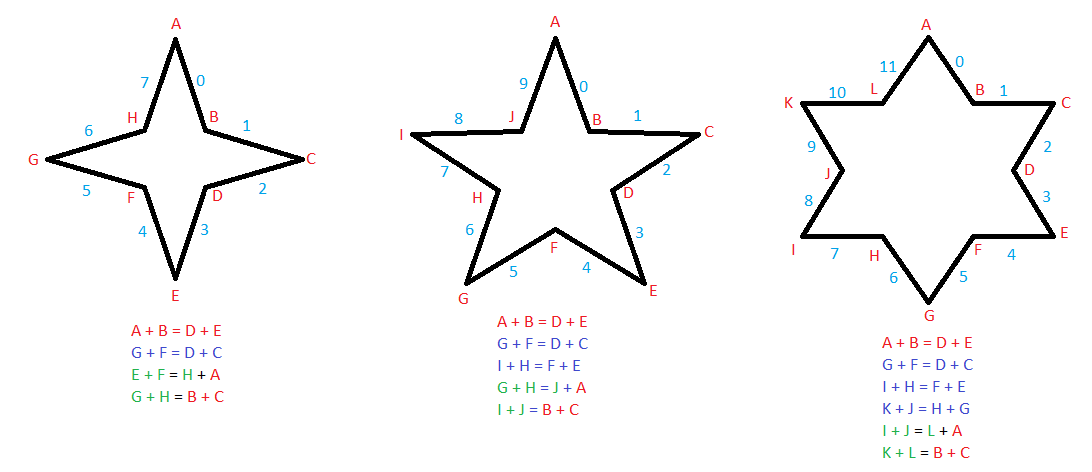
\includegraphics[width=\textwidth]{images/star_analysis.png}
\caption{Esquema descritivo da implementação de restrições} \label{fig:descricao_restricoes}
\end{figure}

Na Figura \ref{fig:descricao_restricoes}, tendo em atenção que as letras representam os operandos e os números os operadores, é possível perceber quais são as restrições fixas e quais as que variam com a dimensão da estrela. As restrições fixas encontram-se a vermelho, a verde estão as restrições que são fixas com o aumento do tamanho, ou seja, são letras que se encontram sempre no mesmo índice relativo na lista de operandos, e a azul as restrições que são acrescentadas com o acréscimo de uma ponta, sendo também visível que se tornam fixas na dimensão acima. Foi com esta análise que foi implementado o predicado growing\_restrictions/3.

% Table generated by Excel2LaTeX from sheet 'Folha1'
\begin{table}[htbp]
  \centering
  \caption{Tempo de execução e número de soluções obtidas com diferentes dimensões}
    \begin{tabular}{lrr}\hline
    \textbf{N º de pontas} & \multicolumn{1}{l}{\textbf{Tempo de Execução(ms)}} & \multicolumn{1}{l}{\textbf{Número de soluções obtidas}} \\ \hline
    \textbf{3 unrestricted} & 563   & 264 \\
    \textbf{3 restricted} & 136   & 132 \\
    \textbf{4 unrestricted} & 15846 & 738 \\
    \textbf{4 restricted} & 3424  & 186 \\
    \textbf{5 unrestricted} & 558125 & 5071 \\
    \textbf{5 restricted} & 80254 & 838 \\
    \textbf{6 unrestricted } & 23416725 & 66334 \\
    \textbf{6 restricted} & 2270679 & 15703 \\ \hline
    \end{tabular}%
  \label{tab:tabela_all_solutions}%
\end{table}%


Na Figura \ref{fig:tempo_execucao_todas_solucoes} e na tabela \ref{tab:tabela_all_solutions} é possível verificar que o aumento do tempo de execução é exponencial com o aumento do número de pontas, assim como o número de soluções, visível na figura \ref{fig:numero_solucoes_todas_solucoes} Por esta razão não foram efetuados teste de dimensão superior a 6 pontas.

\subsection{Estratégias de pesquisa}

A eficiência de um programa em lógica com restrições depende tanto de algoritmos de propagação adequados como de heurísticas apropriadas de seleção da próxima variável a instanciar no processo de enumeração e do valor a atribuir a essa variável.

Foram realizados alguns testes com diferentes combinações heurísticas de ordenação de variáveis, seleção de valores e ordenação de valores para a procura da mesma solução: estrela de 5 pontas com restrições.

Os testes abrangeram todas as combinações possíveis de argumentos de labeling, tanto na parte dos operadores como dos operandos. Os resultados obtidos encontram-se nas tabelas  \ref{tab: heuristicas_operadores} e \ref{tab: heuristicas_operandos}  e nos gráficos \ref{fig:tempo_execucao_combinacoes_heuristicas_operadores} e \ref{fig:tempo_execucao_combinacoes_heuristicas}, respetivamente.
%mudar isto

 Nos resultados obtidos para os operandos, observa-se que a configuração de heurísticas que torna a procura mais eficiente é [min, median, up], aproximadamente 33 segundos mais rápido que a configuração predefinida que é [leftmost,step,up], que melhorou o tempo de execução em 42.5\%; conclui-se também que as configurações consideravelmente menos eficientes são as que usam a heurística occurrence e ffc na ordenação de variáveis,  sendo a configuração menos efieciente [occurence, middle, down], tendo demorado cerca de 4 minutos, o que piora o tempo de execução em 68,4\%. Nestes resultados, é notável a diferença entre o uso de diferentes configurações no labeling.
 
 
 Para os operadores, não se verifica grandes diferenças entre o uso de diferentes configurações no labeling. É possível concluir que a configuração [leftmost,enum,up] é a que torna a procura mais eficiente, tendo melhorado o tempo de execução em 12,7\% e que a configuração [min, bisect,up] é a que torna a procura menos eficiente, tendo piorado o tempo de execução em 65,1\%.
 
 


\input{conteudo/conclusões}

\input{conteudo/referências}

\clearpage
\section{Anexos}
\appendix
\section{Tabelas de dados}

\begin{table}[htbp]
  \centering
  \caption{Resultados da procura de uma solução para cada configuração de operadores}
    \begin{tabular}{lrr}\hline
    \textbf{N º de pontas}  &
    \multicolumn{1}{l}{\textbf{Tempo de execução(ms)}} & \multicolumn{1}{l}{\textbf{Número de soluções obtidas}} \\\hline
    \textbf{3 not restricted} & 108   & 264 \\
    \textbf{3 restricted} & 97    & 23 \\
    \textbf{4 not restricted} & 14761 & 397 \\
    \textbf{4 restricted} & 2905  & 70 \\
    \textbf{5 not restricted} & 734696 & 3567 \\
    \textbf{5 restricted} & 100215 & 546 \\\hline
    \end{tabular}%
  \label{tab:onesolution_per_configuration}%
\end{table}%

\begin{longtable}{llll}

\caption{Resultados dos testes de todas as combinações de heurística possíveis para encontrar configurações de operadores} \\

\hline 
\multicolumn{1}{l}{Heurísticas} &
 &
 &
\multicolumn{1}{l}{Tempo(ms)} \\ \hline 
\multicolumn{1}{l}{Ord. Variáveis} & \multicolumn{1}{l}{Sel.Valores} & 
\multicolumn{1}{l}{Ord.Valores} 
&\\ 
\hline
\endfirsthead

\multicolumn{3}{c}%
{{\bfseries \tablename\ \thetable{} -- Continuação da página anterior}} \\
\hline 
\endhead
    \multicolumn{1}{c}{anti first fail} & \multicolumn{1}{c}{bisect} & down  & 1724 \\
          &       & up    & 1588 \\
          & \multicolumn{1}{c}{enum} & down  & 1541 \\
          &       & up    & 2299 \\
          & \multicolumn{1}{c}{median} & down  & 1773 \\
          &       & up    & 2008 \\
          & \multicolumn{1}{c}{middle} & down  & 1582 \\
          &       & up    & 1808 \\
          & \multicolumn{1}{c}{step} & down  & 2082 \\
          &       & up    & 1686 \\
    \multicolumn{1}{c}{ff} & \multicolumn{1}{c}{bisect} & down  & 1562 \\ \hline
          &       & up    & 1931 \\
          & \multicolumn{1}{c}{enum} & down  & 1365 \\
          &       & up    & 1504 \\
          & \multicolumn{1}{c}{median} & down  & 1589 \\
          &       & up    & 2227 \\
          & \multicolumn{1}{c}{middle} & down  & 1633 \\
          &       & up    & 1660 \\
          & \multicolumn{1}{c}{step} & down  & 1824 \\
          &       & up    & 1999 \\
    \multicolumn{1}{c}{ffc} & \multicolumn{1}{c}{bisect} & down  & 1586 \\ \hline
          &       & up    & 1495 \\
          & \multicolumn{1}{c}{enum} & down  & 1547 \\
          &       & up    & 1411 \\
          & \multicolumn{1}{c}{median} & down  & 1529 \\
          &       & up    & 1525 \\
          & \multicolumn{1}{c}{middle} & down  & 1786 \\
          &       & up    & 1569 \\
          & \multicolumn{1}{c}{step} & down  & 1418 \\
          &       & up    & 1521 \\
    \multicolumn{1}{c}{leftmost} & \multicolumn{1}{c}{bisect} & down  & 1573 \\
          &       & up    & 1483 \\
          & \multicolumn{1}{c}{enum} & down  & 1508 \\
          &       & up    & 1327 \\
          & \multicolumn{1}{c}{median} & down  & 1520 \\
          &       & up    & 1403 \\
          & \multicolumn{1}{c}{middle} & down  & 1516 \\
          &       & up    & 1394 \\
          & \multicolumn{1}{c}{step} & down  & 1464 \\
          &       & up    & 1521 \\
    \multicolumn{1}{c}{max regret} & \multicolumn{1}{c}{bisect} & down  & 1601 \\ \hline
          &       & up    & 1790 \\
          & \multicolumn{1}{c}{enum} & down  & 1958 \\
          &       & up    & 1660 \\
          & \multicolumn{1}{c}{median} & down  & 1951 \\
          &       & up    & 2394 \\
          & \multicolumn{1}{c}{middle} & down  & 1881 \\
          &       & up    & 2177 \\
          & \multicolumn{1}{c}{step} & down  & 1808 \\
          &       & up    & 1824 \\ \hline
    \multicolumn{1}{c}{max} & \multicolumn{1}{c}{bisect} & down  & 1775 \\
          &       & up    & 2012 \\
          & \multicolumn{1}{c}{enum} & down  & 1719 \\
          &       & up    & 2255 \\
          & \multicolumn{1}{c}{median} & down  & 1943 \\
          &       & up    & 2124 \\
          & \multicolumn{1}{c}{middle} & down  & 2034 \\
          &       & up    & 2096 \\
          & \multicolumn{1}{c}{step} & down  & 2541 \\
          &       & up    & 1894 \\ \hline
    \multicolumn{1}{c}{min} & \multicolumn{1}{c}{bisect} & down  & 2904 \\
          &       & up    & 4363 \\
          & \multicolumn{1}{c}{enum} & down  & 1741 \\
          &       & up    & 1486 \\
          & \multicolumn{1}{c}{median} & down  & 1922 \\
          &       & up    & 2141 \\
          & \multicolumn{1}{c}{middle} & down  & 1980 \\
          &       & up    & 1678 \\
          & \multicolumn{1}{c}{step} & down  & 1629 \\
          &       & up    & 1457 \\ \hline
    \multicolumn{1}{c}{occurrence} & \multicolumn{1}{c}{bisect} & down  & 1567 \\
          &       & up    & 1553 \\
          & \multicolumn{1}{c}{enum} & down  & 1513 \\
          &       & up    & 1642 \\
          & \multicolumn{1}{c}{median} & down  & 1477 \\
          &       & up    & 1460 \\
          & \multicolumn{1}{c}{middle} & down  & 1516 \\
          &       & up    & 1365 \\
          & \multicolumn{1}{c}{step} & down  & 1664 \\
          &       & up    & 1892 \\
  \label{tab: heuristicas_operadores}%
  
\end{longtable}%


\begin{longtable}{llll}

\caption{Resultados dos testes de todas as combinações de heurística possíveis para encontrar configurações de operandos} \\

\hline 
\multicolumn{1}{l}{Heurísticas} &
 &
 &
\multicolumn{1}{l}{Tempo(ms)} \\ \hline 
\multicolumn{1}{l}{Ord. Variáveis} & \multicolumn{1}{l}{Sel.Valores} & 
\multicolumn{1}{l}{Ord.Valores} 
&\\ 
\hline
\endfirsthead

\multicolumn{3}{c}%
{{\bfseries \tablename\ \thetable{} -- Continuação da página anterior}} \\
\hline 
\endhead

\endfoot

    \multicolumn{1}{c}{anti first fail} & \multicolumn{1}{c}{bisect} & down  & 68110 \\
          &       & up    & 67805 \\
          & \multicolumn{1}{c}{enum} & down  & 110356 \\
          &       & up    & 110528 \\
          & \multicolumn{1}{c}{median} & down  & 100118 \\
          &       & up    & 58400 \\
          & \multicolumn{1}{c}{middle} & down  & 100202 \\
          &       & up    & 58442 \\
          & \multicolumn{1}{c}{step} & down  & 100317 \\
          &       & up    & 58395 \\ \hline
    \multicolumn{1}{c}{ff} & \multicolumn{1}{c}{bisect} & down  & 70404 \\
          &       & up    & 70409 \\
          & \multicolumn{1}{c}{enum} & down  & 72123 \\
          &       & up    & 72317 \\
          & \multicolumn{1}{c}{median} & down  & 79438 \\
          &       & up    & 67557 \\
          & \multicolumn{1}{c}{middle} & down  & 79558 \\
          &       & up    & 68288 \\
          & \multicolumn{1}{c}{step} & down  & 79577 \\
          &       & up    & 67623 \\\hline
    \multicolumn{1}{c}{ffc} & \multicolumn{1}{c}{bisect} & down  & 157914 \\
          &       & up    & 157018 \\
          & \multicolumn{1}{c}{enum} & down  & 166338 \\
          &       & up    & 166124 \\
          & \multicolumn{1}{c}{median} & down  & 185947 \\
          &       & up    & 142456 \\
          & \multicolumn{1}{c}{middle} & down  & 185793 \\
          &       & up    & 142257 \\
          & \multicolumn{1}{c}{step} & down  & 185268 \\
          &       & up    & 142376 \\\hline
    \multicolumn{1}{c}{leftmost} & \multicolumn{1}{c}{bisect} & down  & 76841 \\
          &       & up    & 77075 \\
          & \multicolumn{1}{c}{enum} & down  & 82302 \\
          &       & up    & 82691 \\
          & \multicolumn{1}{c}{median} & down  & 88116 \\
          &       & up    & 77568 \\
          & \multicolumn{1}{c}{middle} & down  & 88070 \\
          &       & up    & 77777 \\
          & \multicolumn{1}{c}{step} & down  & 89105 \\
          &       & up    & 79003 \\\hline
    \multicolumn{1}{c}{max regret} & \multicolumn{1}{c}{bisect} & down  & 76353 \\
          &       & up    & 75964 \\
          & \multicolumn{1}{c}{enum} & down  & 83341 \\
          &       & up    & 83673 \\
          & \multicolumn{1}{c}{median} & down  & 89541 \\
          &       & up    & 75222 \\
          & \multicolumn{1}{c}{middle} & down  & 89612 \\
          &       & up    & 75121 \\
          & \multicolumn{1}{c}{step} & down  & 89937 \\
          &       & up    & 75307 \\\hline
    \multicolumn{1}{c}{max} & \multicolumn{1}{c}{bisect} & down  & 109743 \\
          &       & up    & 109668 \\
          & \multicolumn{1}{c}{enum} & down  & 108344 \\
          &       & up    & 108539 \\
          & \multicolumn{1}{c}{median} & down  & 90090 \\
          &       & up    & 97558 \\
          & \multicolumn{1}{c}{middle} & down  & 90022 \\
          &       & up    & 97293 \\
          & \multicolumn{1}{c}{step} & down  & 90219 \\
          &       & up    & 97639 \\\hline
    \multicolumn{1}{c}{min} & \multicolumn{1}{c}{bisect} & down  & 71441 \\
          &       & up    & 71185 \\
          & \multicolumn{1}{c}{enum} & down  & 94675 \\
          &       & up    & 94997 \\
          & \multicolumn{1}{c}{median} & down  & 100104 \\
          &       & up    & 45466 \\
          & \multicolumn{1}{c}{middle} & down  & 100333 \\
          &       & up    & 45503 \\ 
          & \multicolumn{1}{c}{step} & down  & 100248 \\
          &       & up    & 45662 \\\hline
    \multicolumn{1}{c}{occurrence} & \multicolumn{1}{c}{bisect} & down  & 198288 \\
          &       & up    & 196999 \\
          & \multicolumn{1}{c}{enum} & down  & 233549 \\
          &       & up    & 233531 \\
          & \multicolumn{1}{c}{median} & down  & 248790 \\
          &       & up    & 200385 \\
          & \multicolumn{1}{c}{middle} & down  & 249684 \\
          &       & up    & 200394 \\
          & \multicolumn{1}{c}{step} & down  & 248703 \\
          &       & up    & 200454 \\ \hline
  \label{tab: heuristicas_operandos}%
\end{longtable}%




\section{Gráficos}

\begin{figure}[!h]
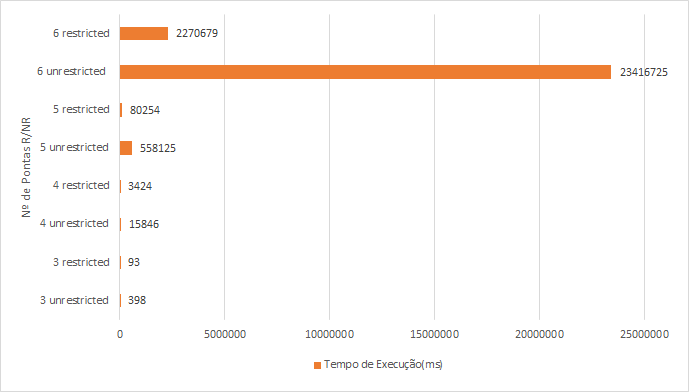
\includegraphics[width=\textwidth]{images/all_solutions_execution_time.png}
\caption{Gráfico correspondente ao tempo de execução da procura de todas as soluções possíveis para diferentes dimensões e restrições} \label{fig:tempo_execucao_todas_solucoes}
\end{figure}

\begin{figure}[!h]
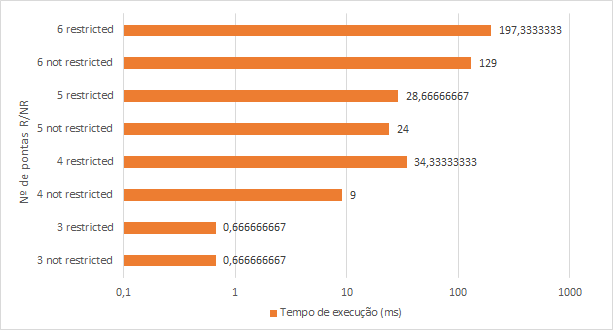
\includegraphics[width=\textwidth]{images/execution_time_random.png}
\caption{Gráfico correspondente ao tempo médio de execução da procura de uma solução para uma configuração de operadores gerada de forma pseudo-aleatória} \label{fig:tempo_execucao_todas_solucoes_random}
\end{figure}

\begin{figure}[!h]
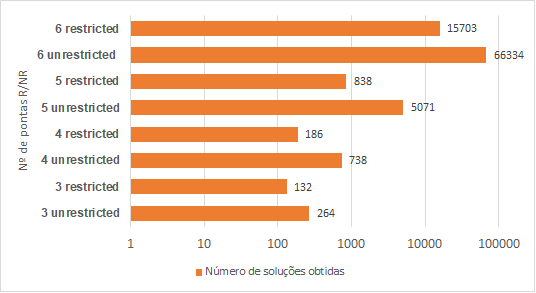
\includegraphics[width=\textwidth]{images/all_solutions_number_tips_r_nr.png}
\caption{Gráfico correspondente ao número de soluções da procura de todas as soluções possíveis} \label{fig:numero_solucoes_todas_solucoes}
\end{figure}

\begin{figure}[!h]
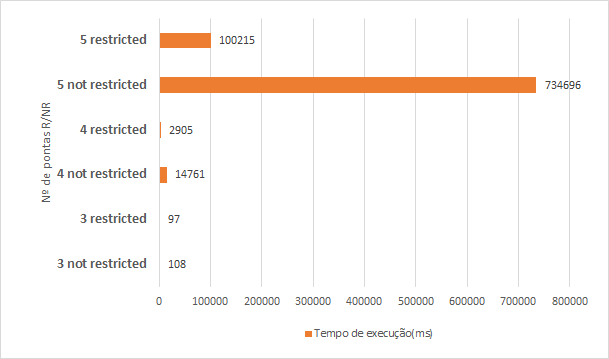
\includegraphics[width=\textwidth]{images/one_solution_each_configuration.png}
\caption{Gráfico correspondente ao tempo de execução da procura de uma solução para cada configuração de operadores} \label{fig:tempo_execucao_uma_solucao}
\end{figure}

\begin{figure}[!h]
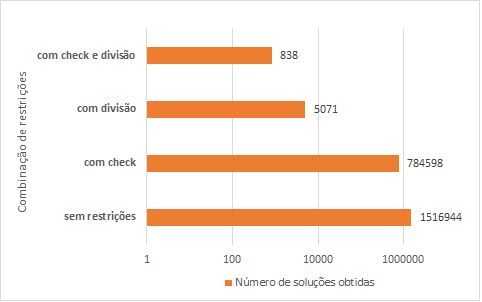
\includegraphics[width=\textwidth]{images/solutions_restriction_combinations.png}
\caption{Gráfico correspondente ao número de soluções para cada combinação de restrições numa estrela de 5 pontas} \label{fig:numero_solucoes_combinacao_restricoes}
\end{figure}

\begin{figure}[!h]
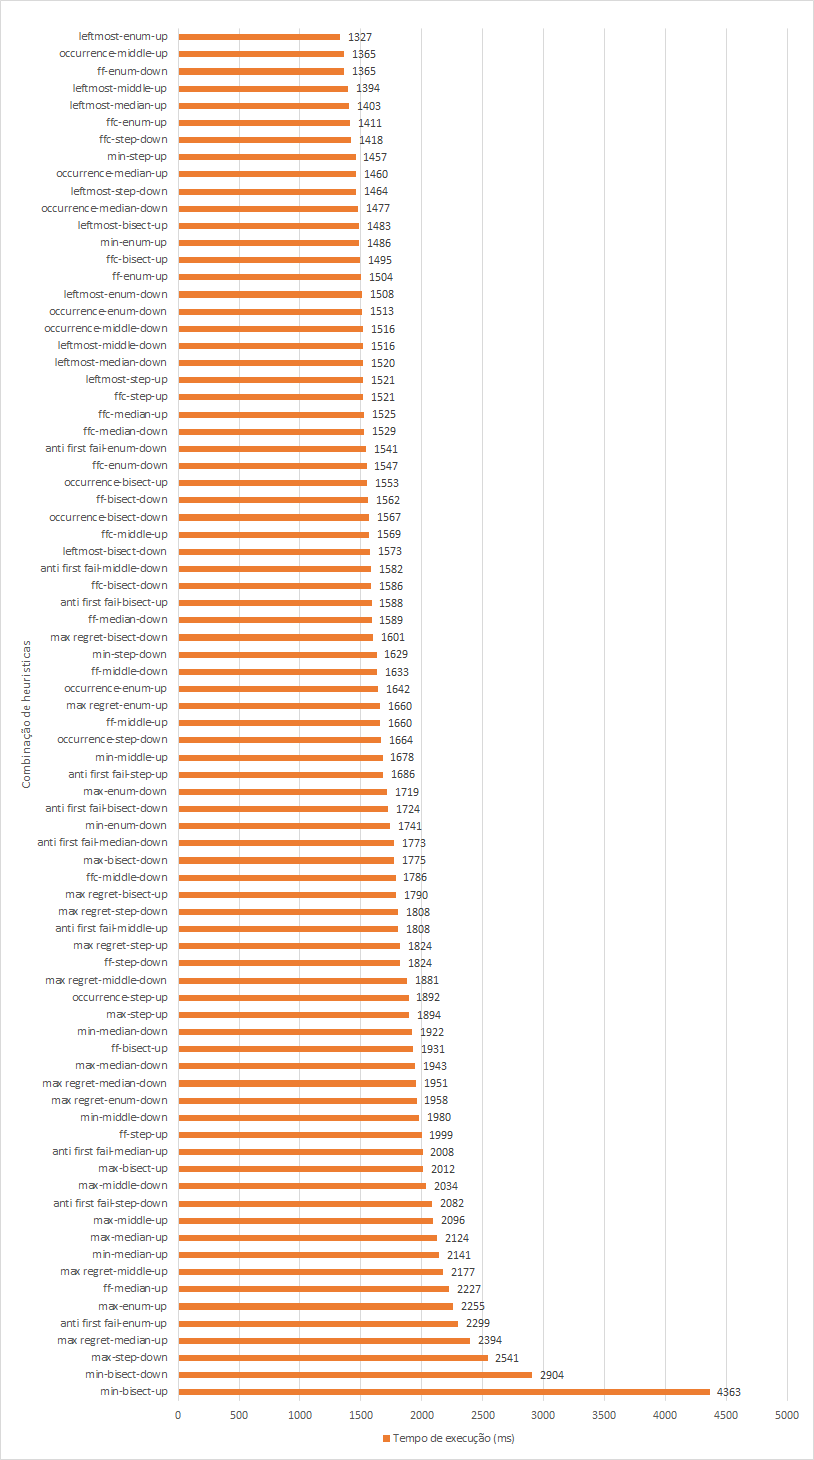
\includegraphics[width=\textwidth]{images/heuristics_ops.png}
\caption{Gráfico correspondente ao tempo de execução da procura restrita de todas as combinações de operadores para cada combinação de heurísticas} \label{fig:tempo_execucao_combinacoes_heuristicas_operadores}
\end{figure}


\begin{figure}[!h]
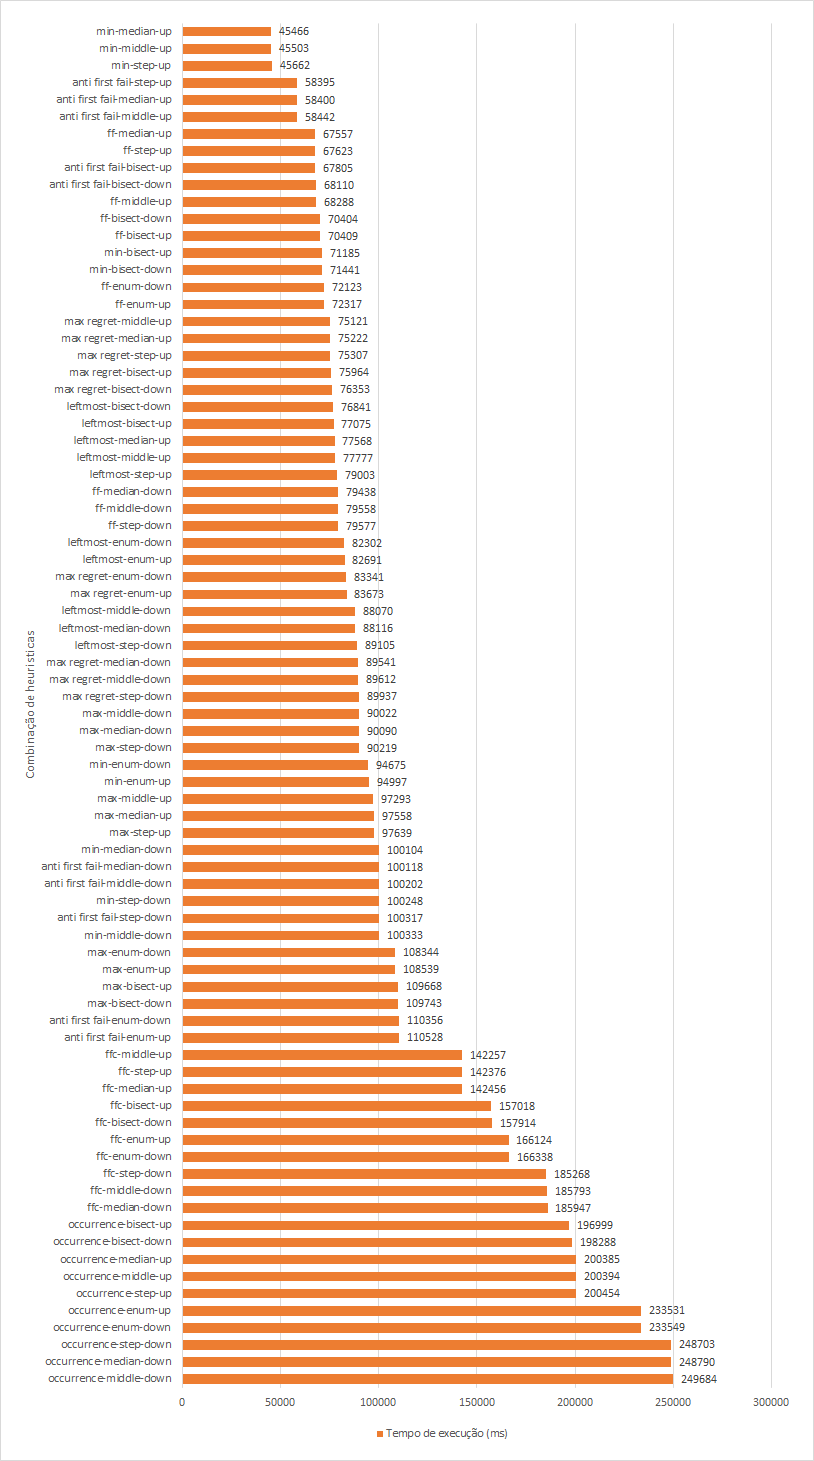
\includegraphics[width=\textwidth]{images/heuristics.png}
\caption{Gráfico correspondente ao tempo de execução da procura restrita de todas as soluções possíveis de uma estrela de 5 pontas para cada combinação de heurísticas} \label{fig:tempo_execucao_combinacoes_heuristicas}
\end{figure}



\end{document}
